\documentclass{article}
\usepackage{tikz}
\usetikzlibrary{positioning, arrows, calc, shapes.multipart}
\usetikzlibrary{decorations.pathreplacing}
\usepackage{amsmath}

\begin{document}

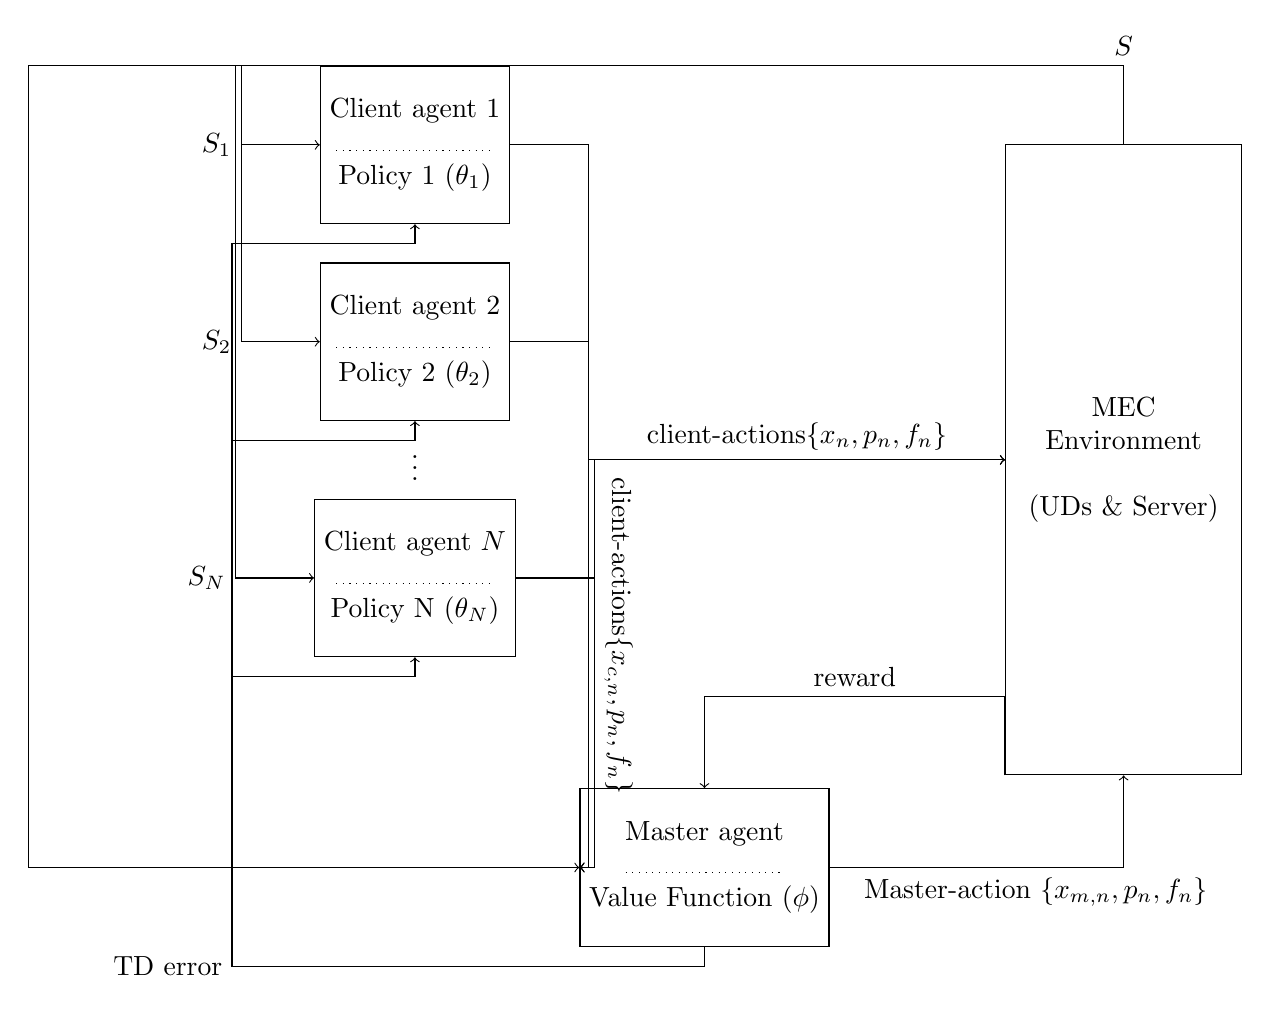
\begin{tikzpicture}[ node distance=2.5cm, every node/.style={align=center}]
  % Nodes
  \node (actor1) [draw, minimum width=1cm, minimum height=2cm, rectangle] {Client agent 1 \\ \tikz \draw[dotted] (0,0) -- (2,0); \\  Policy 1 ($\theta_1$)};
  \node (actor2) [draw, minimum width=1cm, minimum height=2cm, below of=actor1, rectangle] {Client agent 2 \\ \tikz \draw[dotted] (0,0) -- (2,0); \\  Policy 2 ($\theta_2$)};
  \node (actordots) [below of=actor2, node distance=1.5cm] {\vdots};
  \node (actorn) [draw, minimum width=1cm, minimum height=2cm, below of=actordots, node distance=1.5cm, rectangle] {Client agent $N$ \\ \tikz \draw[dotted] (0,0) -- (2,0); \\  Policy N ($\theta_N$)};
  \node (critic) [draw, minimum width=1cm, minimum height=2cm, below right of= actorn, node distance=5.2cm, rectangle] {Master agent\\ \tikz \draw[dotted] (0,0) -- (2,0); \\  Value Function ($\phi$)};
  \node (environment) [draw, minimum width=3cm, minimum height=8cm, right of= actordots, node distance=9cm] {MEC \\Environment \\
  \\(UDs \& Server)};

  % actor arrows
  \draw [->] (actor1.east) -- ++ (0,0cm) -- ++ (1cm,0) |-  (critic.west);
  \draw [->] (actor2.east) -- ++ (0,0cm) -- ++ (1cm,0) |-  (critic.west);
  \draw [->] (actorn.east) -- ++ (0,0cm) -- ++ (1cm,0) |- node[pos=0.1, above, rotate=270, anchor=south] {client-actions{$\{ x_{c,n}, p_n, f_{n}\}$}} (critic.west);
  \draw [->] (actor1.east) -- ++ (1cm,0) |- node[pos=0.75, above] {client-actions{$\{x_{n}, p_n, f_{n}\}$}} (environment.west);
  \draw [->] (actor2.east) -- ++ (1cm,0) |- (environment.west);
  \draw [->] (actorn.east) -- ++ (1cm,0) |- (environment.west);
  \draw [->] (critic.east) -- ++ (1.5cm, 0cm)  -| node[pos=0.25, below] {Master-action {$\{x_{m,n}, p_n, f_{n}\}$}} (environment.south);

  % state arrows
  \draw [->] (environment.north) -- ++(0,1cm) -|node[pos=0, above] {$S$} node[pos=1, left] {$S_1$}([xshift=-1cm]actor1.west) |- (actor1.west);
  \draw [->] (environment.north) -- ++(0,1cm) -|node[pos=1, left] {$S_2$} ([xshift=-1cm]actor2.west) |- (actor2.west);
  \draw [->] (environment.north) -- ++(0,1cm) -|node[pos=1, left] {$S_N$} ([xshift=-1cm]actorn.west) |- (actorn.west);
  \draw [->] (environment.north) -- ++(0,1cm) -| ([xshift=-7cm]critic.west) |- (critic.west);
  \draw [->] (environment.south west) -- ++(0,1cm) -| ([xshift=-0cm]critic.north) node[pos=0.25, above] {reward};

  % TD error
  \draw [->] (critic.south) -- ++(0,-0.25cm) -- ++(-6cm,0) |- ([yshift=-0.25cm] actor1.south) node[pos=0, left] {TD error} -- (actor1.south);
  \draw [->] (critic.south) -- ++(0,-0.25cm) -- ++(-6cm,0) |- ([yshift=-0.25cm] actor2.south) -- (actor2.south);
  \draw [->] (critic.south) -- ++(0,-0.25cm) -- ++(-6cm,0) |- ([yshift=-0.25cm] actorn.south) -- (actorn.south);

\end{tikzpicture}

\end{document}